%%% Local Variables:
%%% mode: latex
%%% TeX-master: "cheat-sheet"
%%% End:

The processors execution of an instruction can be broken down into the following steps~\footnote{\url{http://www.howthecomputerworks.com/cpu/instruction-cycle/}}:
\begin{enumerate}
\item \textbf{Fetch} the instruction From RAM
\item \textbf{Decode} the instruction.
\item \textbf{Execute} the instruction.
\item \textbf{Fetch} any other memory needed to finish the executing the instruction.
\item \textbf{Retire}. Finish and write any memory that needs to be written.
\end{enumerate}

Also simply called the \emph{three-stage pipeline}, if one merges the last three steps. This is also the modern superscalar CPU (see p. 21 in Tanenbaum).

\begin{figure}[H]
  \centering
  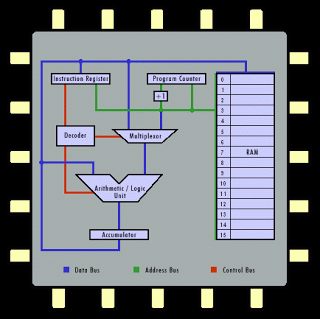
\includegraphics[scale=0.5]{images/cpu}
  \caption{Components of a simple CPU}
\end{figure}

\subsection{Fetch}
The CPU has a spacial register, the \textbf{program counter}, which contains the address of the next instruction to be executed.

After the CPU finishes executing the instruction, the register is updated to point to the next instruction. There is an exception when the CPU executes a branch instruction it will change the instruction pointer register to reflect the new address its supposed to jump to.

\subsection{Decode}
The \emph{decoder} component is responsible for figuring out what the instruction is supposed to do.

\subsection{Execute}
After the decoder sent the instruction to the proper unit, it is now the job of that unit to execute the instruction whatever that instruction maybe. E.g. an \texttt{add} instruction will be sent to the ALU.

\subsection{Fetch some more}
The execution unit may not always have all the necessary data to execute it sometime must fetch other data. This step is not always necessary.

\subsection{Retire}
Store what ever result and update the instruction pointer.
